\section{Deep Learning}

\noindent Wie bereits im vorherigen Kapitel erwähnt, bieten künstliche neuronale Netze die Möglichkeit, komplexe Zusammenhänge in Daten zu erkennen. Um diese Fähigkeit zu erlangen, müssen die Netze jedoch erst gebaut werden. Dies geschieht durch die Bildung neuer Schichten und die Anpassung der Gewichte der einzelnen Neuronen. Zu den frühen Zeiten der künstlichen Intelligenz, wurden neuronale Netze von Menschen wie Algorithmen aufgebaut, was nicht nur die Komplexität der Netze begrenzte, sondern voraussetzte, dass die Entwickler den Lösungsweg mathematisch beschreiben konnten. Besonders bei Themen, wie der Erkennung von Sprache und Gesichtern, die vom Gehirn intuitiv erledigt werden, erwies sich dies als sehr schwer. Deshalb wurde der Prozess des \textit{Deep Learnings} entwickelt. Hier soll das neuronale Netz nicht manuell gebaut werden müssen, sondern baut sich selbst, ähnlich wie es das menschliche Gehirn tut. Um dies zu erreichen, muss das Netz trainiert werden. Hierfür wird eine Sammlung von Ein- und Ausgangswertpaaren an die KI gefüttert, welche anschließend die Gewichte so anpasst, dass die Ausgabe des Netzes möglichst nahe an der gewünschten Ausgabe liegt. Dieser Vorgang wird als \textit{Backpropagation} bezeichnet. Die Differenz zwischen der gewünschten und der tatsächlichen Ausgabe wird berechnet und auf die Gewichte der einzelnen Neuronen zurückgeführt. Die Gewichte werden dann so angepasst, dass die Differenz zwischen gewünschter und tatsächlicher Ausgabe minimiert wird. Dieser Vorgang wird so lange wiederholt, bis die Differenz zwischen gewünschter und tatsächlicher Ausgabe minimal ist. Durch diesen Prozess entstehen eine oder mehrere sogenannte \textit{hidden layers}, abstrakte Schichten, welche die Ein- und Ausgangsschichten miteinander verbinden und die Daten in immer abstraktere Formen umwandeln. Die Anzahl der hidden layers und die Anzahl der Neuronen in diesen Schichten sind frei wählbar. Je mehr hidden layers und Neuronen vorhanden sind, desto komplexere Zusammenhänge können erkannt werden. Dieser Prozess wird in Abbildung \ref{fig:deep_learning} dargestellt. \\

\begin{figure}[H]
    \centering
    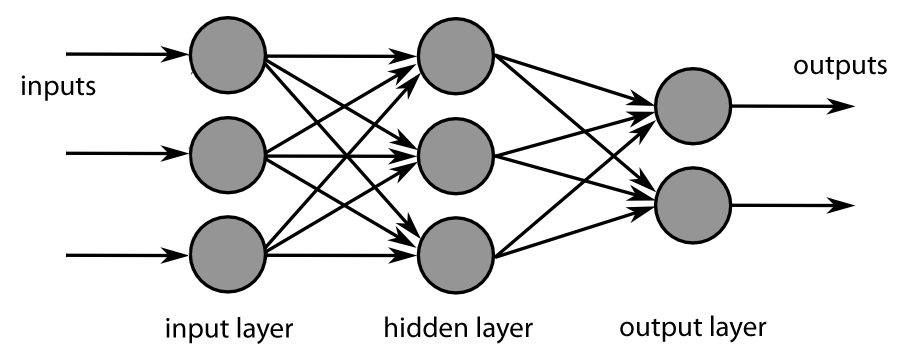
\includegraphics[width=0.6\textwidth]{MultiLayerNeuralNetworkBigger_english.png}
    \caption{Beispiel für neuronales Netz mit einer „hidden layer“} \quelle\url{http://commons.wikimedia.org}
    \label{fig:deep_learning}
\end{figure}

\newpage

%Einsatzgebiete von Deep Learning 